\documentclass[a4paper,11pt]{report}

\usepackage{lscape}
\usepackage{multirow,array}
\usepackage{booktabs}
\usepackage{newunicodechar}
\usepackage{xspace}
\usepackage[francais]{babel}
\renewcommand{\contentsname}{Sommaire}
\usepackage[T1,OT1]{fontenc}
\usepackage{newtxtext,newtxmath}
\usepackage[top=1in, bottom=1in, left=1in, right=1in]{geometry}
\usepackage{amsmath}
\usepackage{amssymb}
\usepackage{listings}
\usepackage{graphicx}
\usepackage{blindtext}
\usepackage{enumitem}
\usepackage{mathtools}
\usepackage{color}
\usepackage[colorlinks=false,hidelinks]{hyperref}
\usepackage{needspace}
\usepackage{pdfpages}
\usepackage{easy-todo}
\usepackage{lipsum}
\usepackage{natbib}
\usepackage{tabularx}
\usepackage{algorithm}
\usepackage[noend]{algpseudocode}
\usepackage{multicol}

%--- custom ---
\newcommand{\solver}{Cbc }

\newcommand{\lang}[1]{\emph{#1}}
\newcommand{\er}{\textsuperscript{er} }
\newcommand{\e}{\textsuperscript{e} }
\newcommand{\ra}[1]{\renewcommand{\arraystretch}{#1}}

\makeatletter
\def\BState{\State\hskip-\ALG@thistlm}
\makeatother

\newcommand{\bin}{\in\{0,1\}}
\newcommand{\real}{\in \mathbb{R}^+}

\definecolor{codegreen}{rgb}{0,0.6,0}
\definecolor{codegray}{rgb}{0.5,0.5,0.5}
\definecolor{codepurple}{rgb}{0.58,0,0.82}
\definecolor{backcolour}{rgb}{0.95,0.95,0.92}
\lstdefinestyle{mystyle}{
    backgroundcolor=\color{backcolour},   
    commentstyle=\color{codegreen},
    keywordstyle=\color{magenta},
    numberstyle=\tiny\color{codegray},
    stringstyle=\color{codepurple},
    basicstyle=\footnotesize,
    breakatwhitespace=false,         
    breaklines=true,                 
    captionpos=b,                    
    keepspaces=true,                 
    numbers=left,                    
    numbersep=5pt,                  
    showspaces=false,                
    showstringspaces=false,
    showtabs=false,                  
    tabsize=2
}
\lstset{style=mystyle}

\DeclareMathOperator{\xor}{XOR}

% --- sectionning ---
\makeatletter
\renewcommand\@chapapp{Partie}

\newcommand\chapterwithsubtitle[2]{
  \chapter[#1: {\itshape#2}]{#1\\[2ex]\Large\itshape#2}
}

\def\@makechapterhead#1{%
  \vspace*{30\p@}%
  {\parindent \z@ \raggedright \normalfont
    \ifnum \c@secnumdepth >\m@ne
        \LARGE\bfseries\thechapter\quad
        %\vskip 20\p@
    \fi
    \interlinepenalty\@M
    \huge \bfseries #1
    %\vskip 40\p@
  }}
\makeatother
\setcounter{tocdepth}{2}


\renewcommand\bibname{Références}
\renewcommand{\refname}{Références}
\makeatletter
\renewcommand\@biblabel[1]{#1.  }
\makeatother

% --- meta data ---
\title{Projet INFO-F-524}
\author{
	Antoine Passemiers \\
	Cédric Simar
}

% --- spec chars ---
\newunicodechar{’}{'}


\begin{document}

\renewcommand\bibname{References}
\renewcommand{\refname}{References}
\makeatletter
\renewcommand\@biblabel[1]{#1.  }
\makeatother

\begin{titlepage}
	\centering
	{\scshape\LARGE Université Libre de Bruxelles\par}
	\vfill
	{\LARGE\bfseries INFO-F-524 \\ Optimisation continue \par
		\vspace{3ex}}
	{\itshape\Large Stochastic Unit Commitment \par}
	\vfill
	\makeatletter
	{\large \@author\par}
	\vfill
	\@date\par
	\makeatother
\end{titlepage}

\tableofcontents

\setlength\parskip{0.5ex plus1ex minus.5ex}


\newpage

\chapter{Introduction}
\vspace*{1.2cm}

TODO Utilisation croissante des énergies renouvelables (solaire et éolienne) 
-> problème de prédictibilité et de contrôle. 
Heureusement, il y a une flexibilité de la demande.

TODO: ajouter organigramme sur le processus de sélection de scenarios.
\chapter{Considérations générales sur l'implémentation}
\vspace*{1.2cm}

Dans le cadre de ce projet, nous avons fait le choix d'utiliser PuLP en tant qu'interface entre
\solver et Python. PuLP est une bibliothèque de modélisation de programmes linéaires et permet
la résolution de ces derniers au moyen de solveurs tels que GLPK, CBC, CLP ou autre.
L'API est stable et largement utilisée, mais contrairement à celle de la bibliothèque CVXPY,
elle ne permet pas de manipuler des variables ou des contraintes de manière vectorisée à l'aide
de matrices ou d'autres structures de données dédiées.

L'implémentation d'une formulation peut de fait devenir fastidieuse et les erreurs difficiles à
retracer lorsque l'on vient à définir des variables multi-indices (implémentables sous forme
de matrices de variables) et indicer ces dernières au sein de boucles. En effet l'absence d'erreur du programme
n'implique pas que les contraintes ont été correctement implémentées et toutes ajoutées au modèle.
Numpy apporte une sécurité supplémentaire relative à la dimensionalité: si par exemple un produit matriciel est effectué
entre une matrice de constantes et un vecteur de variables PuLP et que les dimensions sont incompatibles,
une exception est automatiquement levée. Ceci tient également pour la construction de contraintes où le membre de gauche ne possède pas
la même dimensionalité que le membre de droite, pour la somme de variables, etc.

\section{Extension de PuLP}

Pour les raisons que nous venons de donner, nous avons étendu Numpy afin de rendre l'indiçage 
fantaisiste ("fancy indexing") comptatible avec les variables PuLP. Pour ce faire, nous avons
simplement sous-classé les tableaux \textit{numpy.ndarray} et notamment réécrit les méthodes de comparaison.
La classe fille s'appelle \textit{LpVarArray}. Nous avons entre autres veillé à ce que:
\begin{itemize}
  \item Une combinaison linéaire d'objets \textit{LpVarArray} de dimensions compatibles résultent en un
  un nouvel objet \textit{LpVarArray}.
  \item Une comparaison entre deux \textit{LpVarArray} donne un tableau de contraintes PuLP.
  \item Les tableaux de contraintes PuLP puissent être ajoutés à une instance de problème.
  Pour ce faire, nous avons sous-classé \textit{pulp.LpProblem} en \textit{ArrayCompatibleLpProblem}
  et ajouté les méthodes requises.
\end{itemize}

Motivons nos choix d'implémentation par un exemple concret d'utilisation de ces nouvelles classes.
Supposons que $p$ soit un \textit{LpVarArray} tridimensionnel et $R_plus$ un \textit{numpy.ndarray} contenant 
des constantes. La modélisation peut donc se faire selon deux styles, et nous avons opté pour la seconde
version:
\begin{lstlisting}[language=Python]
    # Ajout séquentiel des contraintes
    for g in range(G):
        for s in range(S):
            for t in range(1, T):
                problem += (p[g, s, t] - p[g, s, t-1] <= R_plus[g])

    # Ajout des contraintes par fancy indexing
    problem += (np.swapaxes(p[:, :, 1:] - p[:, :, :-1], 0, 2) <= R_plus)
\end{lstlisting}

\section{Contenu du dossier source}

Voici comment l'implémentation du projet a été répartie:

\begin{itemize}
  \item \textit{decomposition.py}: Contient l'implémentation de l'unique fonction \textit{decompose\_problem}, permettant
  sur base d'une instance de type \textit{SUPInstance} de générer les instances des problèmes PuLP
  nécessaires, dont le problème original (PP), les sous problèmes issus de la décomposition lagrangienne ($P1_s$ et $P2$),
  ainsi que les problèmes de répartition économique pour chaque scénario ($ED_s$). Tous les problèmes/sous-problèmes
  partagent les variables PuLP, ce qui permet à la résolution d'un problème de \textbf{directement mettre à jour les valeurs
  des variables} dans les problèmes partageant ces mêmes variables, sans que nous ayons explicitement à le faire.
  \item \textit{dive\_and\_fix.py}: Implémentation de l'heuristique dive-and-fix, que nous avons gardé malgré les mauvaises
  performances de celle-ci.
  \item \textit{experimental.py}: Fichier bac à sable
  \item \textit{genetic.pyx}: Implémentation en "pur C" et parallèle d'un algorithme génétique permettant de minimiser
  le nombre de contraintes non satisfaites pour une instance du problème.
  \item \textit{heuristics.py}: Implémentation de \textit{evolve-and-fix} (voir tâche 2).
  \item \textit{instance.py}: Structure de données pour les constantes et indices du problème, accompagnée de fonctions
  utilitaires pour parser les différents fichiers d'instance. Notez la différence entre une instance \textit{SUPInstance}
  telle que définie dans ce fichier, et les instances des problèmes PuLP tels que définis à l'aide de la classe
  \textit{SUCLpProblem} dans le fichier \textit{utils.py}.
  \item \textit{lp\_relaxation.py}: Formulations du problème d'origine ainsi que de sa relaxation linéaire. Selon
  la formulation désirée, le problème est renvoyé sous forme d'une instance de la classe \textit{SUCLpProblem}.
  \item \textit{main.py}: Point d'entrée du programme et parseur de commandes
  \item \textit{subgradient.py}: Algorithme du sous-gradient permettant de trouver une solution duale sur base
  des sous-problèmes $P1_s$ et $P2$.
  \item \textit{utils.py}: Problèmes PuLP et intégration de NumPy dans PuLP telle que décrite dans la section précédente.
  \item \textit{variables.py}: Initialisation des variables nécessaires à la formulation du SUC. Les contraintes spéciales
  (bornes sur les variables) sont implictement ajoutées au problème. Par exemple, les variables $u_{gst}$ sont supposées
  entre comprises entre 0 et 1, et ce peu importe si la formulation choisie est le problème d'origine, la relaxation
  linéaire ou même la décomposition lagrangienne.
\end{itemize}
\chapterwithsubtitle{Tâche 1}{Résoudre la relaxation linéaire de la Formulation SUC}
\vspace*{1.2cm}

\section{Relaxation linéaire}

La relaxation linéaire du modèle utilisé \footnote{A. Papavasiliou. Coupling Renewable Energy Supply with Deferrable Demand. PhD thesis,
University of California, Berkeley, 2011, pg 22} peut être formulée ainsi:\\\\

\begin{tabularx}{\textwidth}{l X r r}
(RL) \hspace{1cm} min \ $\sum\limits_{g \in G} \sum\limits_{s \in S} \sum\limits_{t \in T} \pi_s (K_g u_{gst} + S_g v_{gst} + C_g p_{gst})$ & & (3.20) \\\\
t.q. & \\\\
$\sum\limits_{l \in LI_n} e_{lst} + \sum\limits_{g \in G_n} p_{gst} = D_{nst} + \sum\limits_{l \in LO_n} e_{lst}$ & $\forall n \in N, s \in S, t \in T$ & (3.21) \\
$e_{lst} = B_{ls} (\theta_{nst} - \theta_{mst})$ & $\forall l = (m, n) \in L, s \in S, t \in T$ & (3.22) \\
$e_{lst} \le TC_l$ & $\forall l \in L, s \in S, t \in T$ & (3.23) \\
$-TC_l \le e_{lst}$ & $\forall l \in L, s \in S, t \in T$ & (3.24) \\
$p_{gst} \le P_{gs}^{+} u_{gst}$ & $\forall g \in G, s \in S, t \in T$ & (3.25) \\
$P_{sg}^{-} u_{gst} \le p_{gst}$ & $\forall g \in G, s \in S, t \in T$ & (3.26) \\
$p_{gst} - p_{gs,t-1} \le R_g^{+}$ & $\forall g \in G, s \in S, t \in T$ & (3.27) \\
$p_{gs,t-1} - p_{gst} \le R_g^{-}$ & $\forall g \in G, s \in S, t \in T$ & (3.28) \\
$\sum\limits_{q=t-UT_g+1}^{t} z_{gq} \le w_{gt}$ & $\forall g \in G_s, t \ge UT_g$ & (3.29) \\
$\sum\limits_{q=t+1}^{t+DT_g} z_{gq} \le 1 - w_{gt}$ & $\forall g \in G_s, t \le N - DT_g$ & (3.30) \\
$\sum\limits_{q=t-UT_g+1}^{t} v_{gsq} \le u_{gst}$ & $\forall g \in G_f, t \ge UT_g$ & (3.31) \\
$\sum\limits_{q=t+1}^{t+DT_g} v_{gsq} \le 1 - u_{gst}$ & $\forall g \in G_f, t \le N - DT_g$ & (3.32) \\
$z_{gt} \le 1$ & $\forall g \in G_s, t \in T$ & (3.33) \\
$v_{gst} \le 1$ & $\forall s \in S, t \in T$ & (3.34) \\
$z_{gt} \ge w_{gt} - w_{g,t-1}$ & $\forall g \in G_s, t \in T$ & (3.35) \\
$v_{gst} \ge u_{gst} - u_{gs,t-1}$ & $\forall g \in G_f, s \in S, t \in T$ & (3.36) \\
$\pi_s u_{gst} = \pi_s w_{gt}$ & $\forall g \in G_s, s \in S, t \in T$ & (3.37) \\
$\pi_s v_{gst} = \pi_s z_{gt}$ & $\forall g \in G_s, s \in S, t \in T$ & (3.38) \\
$p_{gst} \ge 0, \ 0 \le u_{gst} \le 1$ & $\forall g \in G, s \in S, t \in T$ & (3.39) \\
$z_{gt} \ge 0, \ 0 \le w_{gt} \le 1$ & $\forall g \in G_s, t \in T$ & (3.40) \\
\end{tabularx}

\vspace{2cm}

\subsection{Incertitudes du modèle}

\begin{itemize}
    \item Les contraintes (3.21) d'équilibre de marché imposent que la production d'énergie satisfasse la demande étant donné les niveaux de puissance
    assignés aux lignes de transmission.
    \item Les contraintes (3.22) sont obtenues à partir de la première loi de Kirchhoff (loi des noeuds) et de la seconde loi de Kirchhoff
    (loi des mailles). La susceptance y sert à modéliser la puissance lorsque les lignes sont parcourues par un courant continue.
    Les lignes du réseau peuvent être soumises à des contingences, symbolisées par les susceptances des lignes.
    Lorsqu'une ligne de transmission $l$ est mise hors service dans un scénario $s$, la susceptance associée $B_{ls}$ est fixée à 0.
    \item Les contraintes de types (3.25) et (3.26) tiennent compte des contingences liées aux générateurs eux-mêmes.
    Dans tout scénario $s$ où un générateur $g$ est hors usage, les constantes $P_{gs}^{+}$ et $P_{gs}^{-}$ sont fixées à 0 afin de forcer
    la production à 0.
\end{itemize}

\subsection{Non-anticipativité}

Les contraintes (3.37) et (3.38) de non-anticipativité permettent de forcer la planification des générateurs lents établie lors de la seconde phase
à respecter celle effectuée pour ces mêmes générateurs lors de la première phase. En effet les contingences peuvent être énumérées (d'où la présence
de scénarios) mais ne peuvent avoir de caratère certain. L'engagement des générateurs lents doit donc être le même dans tous les scénarios,
d'où les contraintes d'égalité. Étant donné que les variables $w_{gt}$ et $z{gt}$ sont définies pour les générateurs lents
et les variables $u_{gst}$ et $v_{gst}$ pour tous les générateurs, $u_{gst}$ et $v_{gst}$ sont redondantes pour les générateurs lents.

Cette redondance n'est justifiée que par l'utilisation de la relaxation lagrangienne et la dualisation des contraintes de non-anticipativité, car
elle permet de borner les sous-problèmes produits par la décomposition lagrangienne. En l'absence d'une telle relaxation il convient alors de retirer 
de la modélisation les variables $u_{gst}$ et $v_{gst}$ associées aux générateurs lents. Puisque nous avons gardé la même approche qu'Anthony Papavasiliou
pour la décomposition lagrangienne, toutes les variables ont été gardées.

\subsection{Démarrage des générateurs et contraintes temporelles}

Les contraintes de type (3.35) et (3.36) couplent des variables liées à des périodes de temps adjacentes.
Par exemple, les contraintes de type (3.35) sont définies $\forall t \in T$. Or les valeurs des variables
$w_{gt}$ ne sont pas connues pour $t = 0$. Nous n'avons pas fait l'hypothèse que les générateurs en question
sont éteints en $t = 0$, et simplement retiré la première contrainte. Les contraintes sont donc définies
$\forall t \in T \backslash \{0\}$, ce qui simplifie le problème et allège légèrement les temps d'exécution.

\chapterwithsubtitle{Tâche 2}{Développer une heuristique qui trouve une solution entière admissible}
\vspace*{1.2cm}

\section{Algorithme génétique}



\section{TODO}

\begin{figure}[h!]
    \begin{center}
        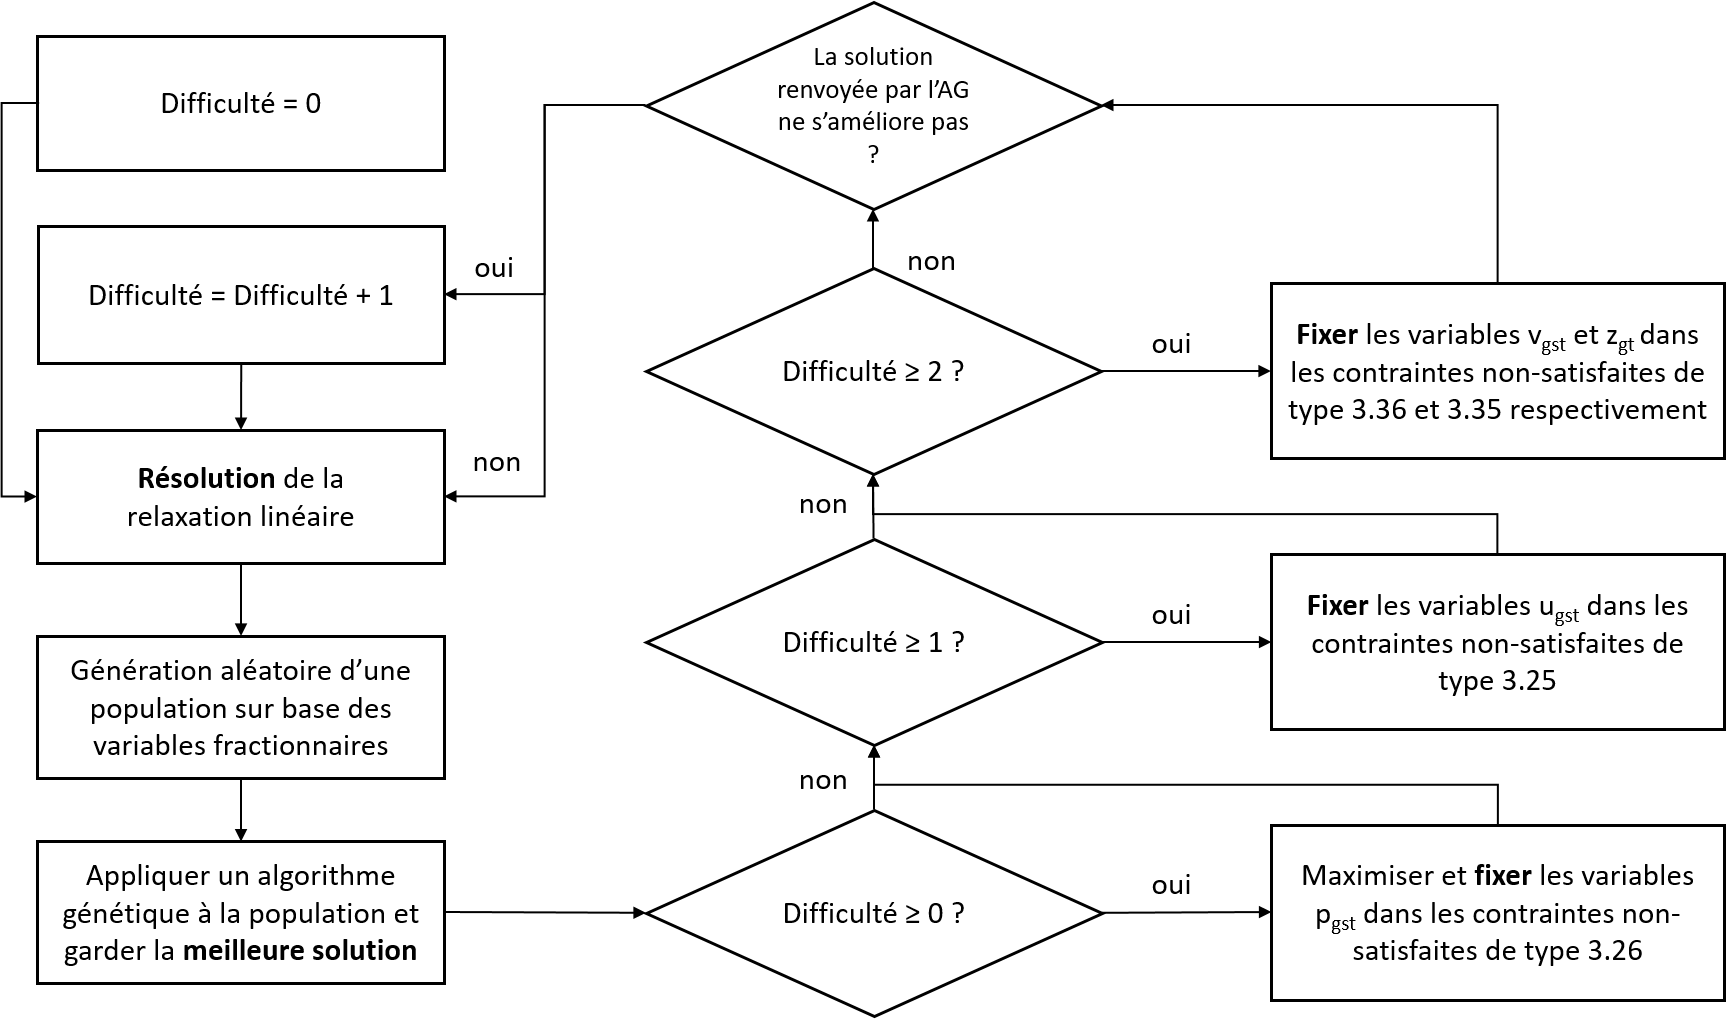
\includegraphics[width=\textwidth]{imgs/evolveandfix.png}\\
        Vue générale de l'algorithme proposé "evolve-and-fix"
    \end{center}
\end{figure}
\chapterwithsubtitle{Tâche 3}{Résoudre une relaxation Lagrangienne de la Formulation SUC}
\vspace*{1.2cm}

\section{Décomposition lagrangienne}

Le choix des contraintes relâchées est le même que celui effectué par A. Papavasiliou:
seules les contraintes de non-anticipitavité ont été dualisées. Les deux raisons
principales sont que d'une part elles compliquent fortement le problème à résoudre
et que d'autre part, elles sont les seules contraintes à coupler les différents
scénarios entre eux. Sans elles, \textit{il est désormais possible de décomposer le problème
suivant ses différents scénarios}.

Enfin, la relaxation de ses contraintes seules est suffisante pour diminuer significativement
le temps d'exécution du solveur. En particulier, la somme des temps d'exécution sur les
différents sous-problèmes créés est fortement inférieure au temps d'exécution sur le problème
primal, et ceci est d'autant plus valable pour les instances de grande taille.

Le dual lagrangien est donc obtenu en reprenant la fonction objectif du primal et en y
dualisant les contraintes de non-anticipativité $(3.37)$ et $(3.38)$:

\begin{align*}
    \mathcal{L} & = \sum\limits_{g \in G} \sum\limits_{s \in S} \sum\limits_{t \in T} \pi_s (K_s u_{gst} + S_g v_{gst} + C_g p_{gst}) + \sum\limits_{g \in G_s} \sum\limits_{s \in S} \sum\limits_{t \in T} \pi_s (\mu_{gst} (u_{gst} - w_{gt}) + \nu_{gst} (v_{gst} - z_{gt})) \\
    & = \sum\limits_{s \in S} \Big(\sum\limits_{g \in G} \sum\limits_{t \in T} (K_s u_{gst} + S_g v_{gst} + C_g p_{gst}) + \sum\limits_{g \in G_s} \sum\limits_{t \in T} \pi_s (\mu_{gst} u_{gst} + \nu_{gst} v_{gst})\Big) \\
    & - \sum\limits_{g \in G_s} \sum\limits_{s \in S} \sum\limits_{t \in T} \pi_s (\mu_{gst} w_{gt} + \nu_{gst} z_{gt}) \\
\end{align*}

Nous observons qu'en réarrangeant les termes de la fonction il est possible de l'exprimer sous la forme d'une somme de plusieurs objectifs, 
dont un est indépendant du scénario et chacun des autres est assigné à un scénario $s$.
La décomposition lagrangienne se fait alors comme suit:

\begin{itemize}
    \item \textbf{Les sous-problèmes P1$_{\text{s}}$} concernent la plannification des générateurs rapides.
    Le sous-problème $P1_s$ requiert de plannifier les générateurs rapides dans le cadre du scénario $s$.
    La fonction objectif est donnée par \citep{Papavasiliou2013}:
    \begin{equation}
        \min \ \sum\limits_{g \in G} \sum\limits_{t \in T} (K_s u_{gst} + S_g v_{gst} + C_g p_{gst}) + \sum\limits_{g \in G_s} \sum\limits_{t \in T} \pi_s (\mu_{gst} u_{gst} + \nu_{gst} v_{gst})
    \end{equation}
    \item \textbf{Le sous-problème P2} concerne la plannification des générateurs lents et ne prend donc pas
    en considération les différents scénarios. La valeur de son objectif est quant à elle donnée par:
    \begin{equation}
        \min \ - \sum\limits_{g \in G_s} \sum\limits_{s \in S} \sum\limits_{t \in T} \pi_s (\mu_{gst} w_{gt} + \nu_{gst} z_{gt})
    \end{equation}
\end{itemize}

La valeur de l'objectif du dual lagrangien est donc exprimé sous la forme d'une somme des objectifs des différents sous-problèmes
issus de cette décomposition. La tâche consiste à présent à optimiser le dual lagrangien afin de rapprocher la solution duale de la
zone admissible du primal.

\section{Optimisation du dual lagrangien}

\subsection{Choix de l'algorithme}

Comme expliqué par A. Papavasiliou dans une présentation de 2016 \citep{Asynchronous},
il est possible que certains sous-problèmes $P1_s$ prennent considérablement plus de temps que le autres pour être résolus, \textit{jusqu'à
75 fois le temps pris par le sous-problème le plus rapide}. Ceci crée des goulots d'étranglement lors de l'optimisation du dual,
qui peuvent cependant être résolus par l'utilisation d'un algorithme d'optimisation asynchrone.
En particulier, l'\textit{algorithme de descente par blocs} a été présenté et permet de mettre à jour un sous-ensemble des multiplicateurs
lagrangiens en calculant une partie du sous-gradient à la fois. Ce fragment est le sous-ensemble de composantes associées à un seul
scénario. L'algorithme se distingue donc des algorithmes de descente par coordonnée car plusieurs variables duales sont mis à jour
à la fois.

Nous avons eu la chance de ne pas observer de tels ralentissements pour les instances fournies et les temps de résolution des différents
sous-problèmes étaient fort similaires. En conséquence, nous avons fait le choix d'utiliser l'\textit{algorithme du sous-gradient} car il est
plus simple à implémenter que l'algorithme de descente par blocs.
Le sous-gradient $d^k$ associés aux multiplicateurs lagrangiens à l'itération $k$ est donné par:
\begin{align}
    d_{\mu_{gst}}^k = & \ \pi_s (w_{gt}^k - u_{gst}^k) \ \  \forall g \in G_s, s \in S, t \in T \\
    d_{\nu_{gst}}^k = & \ \pi_s (z_{gt}^k - v_{gst}^k) \ \  \forall g \in G_s, s \in S, t \in T
\end{align}
où $d_{\mu}^k$ est le partie du sous-gradient associée aux contraintes $(3.37)$ et $d_{\nu}^k$ est celle associée aux contraintes $(3.38)$.
Il est important de noter que \textbf{les multiplicateurs lagrangiens sont mis à jour à l'aide de l'équation décrite dans cette même présentation
et non celle présentée dans la thèse} \citep{Papavasiliou12couplingrenewable} (il s'agit selon nous d'une simple erreur de signe).
Les multiplicateurs lagrangiens sont donc calculés d'itération en itération de la façon suivante:
\begin{align}
    \mu_{gst}^{0} & = 0 \ \  \forall g \in G_s, s \in S, t \in T \\
    \nu_{gst}^{0} & = 0 \ \  \forall g \in G_s, s \in S, t \in T \\
    \mu_{gst}^{k+1} & = \ \mu_{gst}^{k} - \alpha_k d_{\mu_{gst}}^k \ \  \forall g \in G_s, s \in S, t \in T \\
    \nu_{gst}^{k+1} & = \ \nu_{gst}^{k} - \alpha_k d_{\nu_{gst}}^k \ \  \forall g \in G_s, s \in S, t \in T
\end{align}
L'étape suivante est donc de trouver un pas $\alpha_k$ assurant une convergence de l'algorithme.


\subsection{Calcul du pas}

Un pas de déplacement fortement utilisé en pratique, décrit par Fisher et Held notamment, repris par Papavasiliou, est décrit ainsi:
\begin{equation}
    \alpha^k = \frac{\lambda (\hat{L} - L^k)}{\sum\limits_{g \in G_s} \sum\limits_{s \in S} \sum\limits_{t \in T} \big(\pi_s^2 \ (u_{gst}^k - w_{gt}^k)^2 + \pi_s^2 \ (v_{gst}^k - z_{gt}^k)^2\big)}
\end{equation}
où $\lambda$ est un paramètre constant, $\hat{L}$ est une borne supérieure sur la solution optimale du primal et $L^k$ est la somme des objectifs des sous-problèmes
à l'itération $k$. Il reste donc le problème de trouver une borne supérieure raisonnable sur la valeur de la solution optimale,
et que l'on puisse calculer rapidement. Il reste encore à calculer une borne supérieure, qui peut être trouvée notamment avec une solution primale faisable.
Le problème est que trouver une solution faisable constitue déjà une difficulté. Puisque l'obtention d'une solution primale faisable
concerne la tâche 4 du projet, nous avons décidé de \textbf{nous affranchir de ce problème dans le cadre de la tâche 3}.
Nous n'avons donc pas pris en considération l'idée de Papavasiliou consistant en l'obtention d'une solution faisable par résolution
du problème de répartition économique (\textit{economic dispatch}).
Deux autres raisons à ce choix est qu'une telle solution ne peut être obtenue que vers les dernières itérations du sous-gradient
(nous laissant donc sans borne supérieure durant la majorité du temps d'exécution), et que la résolution des différents sous-problèmes
de répartition économique (un par scénario) ralentit le sous-gradient, malgré le fait que les différents sous-problèmes peuvent être résolus en parallèle.
Pour cette tâche nous avons opté pour une alternative plus simple inspirée de \citep{Zhuang1988}.
La méthode a été montrée comme efficace sur le problème de \textit{unit commitment} et calcule le pas de déplacement uniquement
sur base de deux paramètres de contrôle et du numéro de l'itération courante. Dans l'article en question le pas est mis à jour de la façon suivante:
\begin{equation}
    \alpha^k = \frac{1}{\alpha + \beta k} \ , \  \alpha, \beta > 0
\end{equation}
Dans l'implémentation de notre sous-gradient, nous avons plutôt utilisé la formule suivante:
\begin{equation}
    \alpha_k = \alpha_0 \rho^k
\end{equation}
où $\alpha_0$ et $\rho$ doivent être choisis suffisamment grands afin d'assurer la convergence de l'algorithme.
\chapterwithsubtitle{Tâche 4}{Développer une heuristique basée sur la solution obtenue par la relaxation de la tâche précédente}
\vspace*{1.2cm}

Contrairement à ce qui a été suggéré dans l'énoncé et malgré l'utilité que peuvent avoir les multiplicateurs lagrangiens
dans la recherche d'une solution primale admissible, nous avons choisi d'exploiter exclusivement l'information
contenue dans l'historique des solutions primales non-admissibles obtenues avec la méthode du sous-gradient.
En effet, beaucoup d'auteurs dont \citep{doi:10.1137/S1052623498332336} et \citep{Zhuang1988}
suggèrent de rapprocher d'avantage la solution courante de la zone admissible du primal en calculant une combinaison
convexe des différentes solutions obtenues pour le primal.

\section{Séquences ergodiques}

Nous définissons une séquence ergodique comme étant une série $\{\overline{x}^k\}$ où l'élement $\overline{x}^k$
est calculé ainsi \citep{Aldenvik}:
\begin{equation}
    \overline{x}^k = \sum\limits_{s=0}^{t-1} \mu_s^t x^s \ , \ \sum\limits_{s=0}^{t-1} \mu_s^t = 1 \ , \ \mu_s^t \le 0 \ , \ s = 0, \ldots, t-1
\end{equation}
où $x^s$ est une solution primale infaisable obtenue à l'itération $s$ de l'algorithme du sous-gradient et $\mu_s^t x^s$ est un coefficient
de la combinaison convexe $\overline{x}^k$. La nouvelle solution primale obtenue à l'itération $t$ est donc bien une combinaison convexe 
des solutions déjà obtenues.

Andrea Simonetto et Hadi Jamali-Rad~\citep{Simonetto2016} fournissent une preuve de convergence forte de cette série.
En revanche, la combinaison des variables binaires de notre problème ont de grandes chances de \textbf{générer des valeurs fractionnaires} pour
celles-ci. Il a été montré que ce nombre de valeurs fractionnaires est fortement réduit lorsque le nombre d'unités dans le problème
est significativement supérieur au nombre de périodes de temps. Cependant ceci n'est pas notre cas et il est nécessaire de recourir à une 
méthode de recherche locale afin de trouver une solution respectant les contraintes d'intégralité.
La convergence forte n'est pas assurée mais cependant dans le cas d'un problème entier (binaire) mixte (ce qui est le cas), la série converge vers 
un point de l'enveloppe convexe de la zone admissible. Beaucoup d'auteurs interprètent les valeurs fractionnaires comme des probabilités
d'occurence: $u_{gst}$ peut par exemple être vu comme la probabilité que le générateur $g$ soit actif lors de la période $t$ dans le scénario $s$.
Comme méthode de recherche locale, nous avons simplement utilisé \textbf{l'heuristique implémentée dans le cadre de la tâche 2} car nous l'avons
justement spécialement conçue pour les solutions contenant des valeurs fractionnaires.

\section{Bornes supérieures}

L'algorithme tel qu'implémenté dans la tâche 3 a été modifié afin de calculer une borne supérieure sur base de solution primales admissibles.
Cependant, au début de la méthode du sous-gradient, les solutions duales trouvées génèrent des solutions primales
correspondantes fort éloignée de la zone admissible: il y a donc de plus grandes choses de voir l'heuristique échouer.
Nous introduisons un paramètre \textit{$n_{ar}$} correspondant au nombre d'itérations du sous-gradient avant de commencer à utiliser
l'heuristique pour reconstruire une solution du primal. Lorsqu'une première solution admissible est trouvée, la borne supérieure est abaissée
à la valeur de l'objectif trouvé et le pas du sous-gradient est calculé sur base des bornes supérieures et inférieures.
Tant qu'aucune solution admissible n'est disponible, le pas est calculé via la suite géométrique décrite à la fin de la tâche 3.

\subsubsection{Calcul du pas sur base d'une borne supérieure}

Une façon naïve de calculer une borne supérieure rapidement est de fixer les variables
$u_{gst}, v_{gst}, p_{gst}$ $\ \forall g \in G, s \in S, t \in T$ à leurs valeurs maximales respectives.
Il est assez clair que la solution correspondante devient infaisable et que seules les contraintes 
$(3.25), (3.33), (3.34), (3.39), (3.40)$ sont garanties d'être satisfaites. Par exemple, certaines contraintes $(3.36)$ cessent d'être satisfaites
car il n'est pas possible d'allumer un générateur deux fois d'affilée. Cependant, la valeur de l'objectif constitue une borne supérieure
car toute solution faisable nécessite d'abaisser la valeur d'une des variables $u_{gst}, v_{gst}, p_{gst} \ \forall g \in G, s \in S, t \in T$
afin de satisfaire les contraintes restantes. En revanche cette borne est très mauvaise et \textbf{peut atteindre une valeur considérablement plus grande que l'objectif de la solution optimale}.
Cette borne $WUB$ est calculée ainsi:
\begin{equation}
    WUB = \sum\limits_{g \in G} \sum\limits_{s \in S} \sum\limits_{t \in T} \pi_s (K_g + S_g + C_g P_{gs}^{+})
\end{equation}

Cette borne supérieure a été utilisée lors de l'implémentation du sous-gradient de la tâche 3 et a été abandonnée au profit de la suite géométrique et
des objectifs des solutions primales trouvées heuristiquement.

\section{Vue générale de la méthode}

\begin{algorithm}[H]
\caption{Méthode du sous-gradient pour le problème SUC}
\begin{algorithmic}[1]
\Procedure{solve\_with\_subgradient}{}
\State $k \leftarrow 0$
\State $UB \leftarrow WUB, \ LB \leftarrow -\infty$ 
\State $\mu_{gst} \leftarrow 0 \ , \ nu_{gst} \leftarrow 0 \ \ \forall g \in G, s \in S, t \in T$
\While {$\frac{(UB - LB)}{UB} \le \epsilon$}
\State Résoudre les sous-problèmes $P2$ et $P1_s \ \forall s \in S$
\State $L_k \leftarrow $ \ somme des objectifs des différents sous-problèmes
\If {$L_k = LB$}
\State $\lambda \leftarrow \lambda / 2$
\EndIf
\If {$L_k > LB$}
\State $LB \leftarrow L_k$
\EndIf
\If {$k > n_{ar}$}
\State Somme ergodique $\overline{x}^k$ de toutes les solutions primales infaisables obtenues
\State Obtenir une solution primale admissible de manière heuristique depuis $\overline{x}^k$
\EndIf
\If {$\hat{L} < UB$}
\State $UB \leftarrow \hat{L}$
\EndIf
\If {$k > n_{ar}$ et une solution admissible a été trouvée}
\State $\alpha_k = \frac{\lambda (\hat{L} - L^k)}{\sum\limits_{g \in G_s} \sum\limits_{s \in S} \sum\limits_{t \in T} \big(\pi_s^2 \ (u_{gst}^k - w_{gt}^k)^2 + \pi_s^2 \ (v_{gst}^k - z_{gt}^k)^2\big)}$
\Else
\State $\alpha_k = \alpha_0 \ \rho^k$
\EndIf
\State Mise à jour des multiplicateurs $\mu_{gst}, \nu_{gst} \ \ \forall g \in G, s \in S, t \in T$
\State $k \leftarrow k + 1$
\EndWhile
\EndProcedure
\end{algorithmic}
\end{algorithm}
\chapterwithsubtitle{Tâche 5}{Comparer les meilleures solutions obtenues (optimum et temps de résolution) avec les heuristiques, par rapport à celle trouvées avec la relaxation choisie}
\vspace*{1.2cm}


\section{Convergence d'evolve-and-fix (tâche 2)}

Comme expliqué dans la partie portant sur la tâche 2 du projet, 
l'heuristique proposée fonctionne principalement sur des instances de très petite
taille et nécessite de fixer les variables de manière plus stratégique afin
d'éviter de violer les contraintes liées aux démarrages des générateurs
(de type 3.32 entre autres).

\begin{figure}[h!]
\begin{center}
	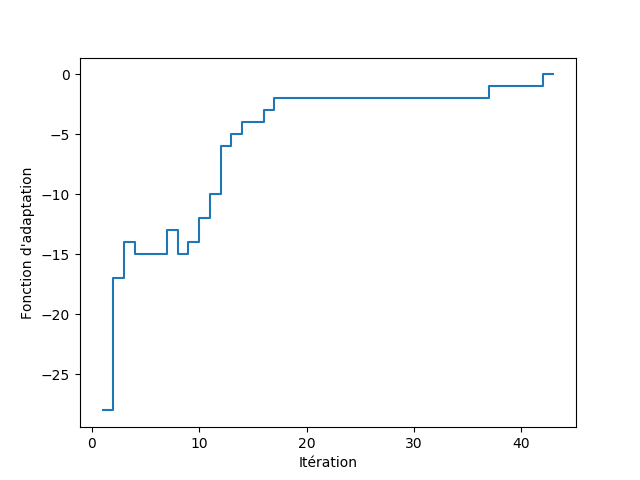
\includegraphics[width=.5\textwidth]{imgs/round}
	\caption{\'Evolution de la fonction d'adaptation calculée par evolve-and-fix
    sur l'instance \textit{inst-10-6-5-0.txt} - Méthode d'arrondi de la solution
    obtenue par la relaxation linéaire: Pour cette l'instance, le nombre de contraintes
    non satisfaites tombe rapidement à 0, permettant à l'heuristique de renvoyer
    une solution admissible.}
\end{center}
\end{figure}

Cependant, l'heuristique a l'avantage de ne posséder aucun paramètre si ce n'est ceux
de l'algorithme génétique, qui quant à eux peuvent être laissés à leurs valeurs par
défaut. En effet, les résultats obtenus sont fort robustes à l'ajustement des paramètres.
Les valeurs par défaut sont les suivantes:
\begin{itemize}
    \item Taille de la population: 100
    \item Nombre d'individus lors d'un tournoi: 2
    \item Taux de mutation: 2
    \item Nombre maximum d'itérations: 100000
\end{itemize}

\section{Convergence du sous-gradient (tâches 3 et 4)}

Il est important de noter qu'evolve-and-fix trouve une solution plus aisément lorsqu'appliqué
à une solution proche de la zone admissible, en particuler la somme ergodique d'une (de préférence
longue) série de solutions primales non-faisables.

\begin{figure}[h!]
\begin{center}
    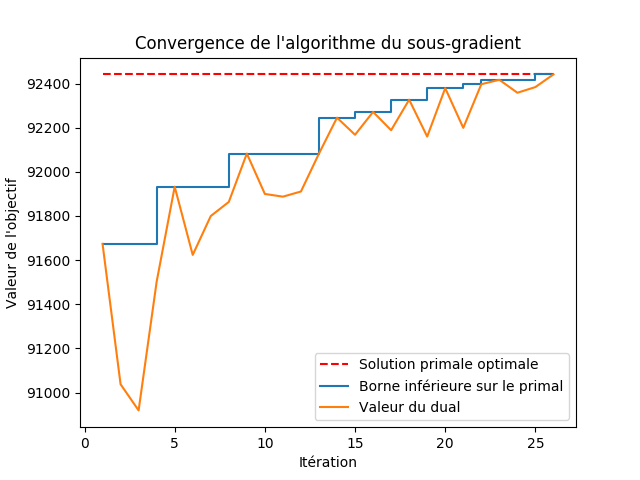
\includegraphics[width=.5\textwidth]{imgs/subgradient}
    \caption{Convergence du sous-gradient pour l'instance \textit{inst-10-6-5-0.txt}:
    Pour cette instance, la solution optimale du primal a été retrouvée.}
\end{center}
\end{figure}

Sur les plus petites instances fournies, le temps requis pour trouver la solution optimale du problème
d'origine (sans relaxation ni heuristique) est largement inférieur à celui pris par le sous-gradient
pour converger et trouver la solution optimale. Ce phénomène s'estompt rapidement lorsque la taille
du problème augmente (que ce soit par son nombre de scénarios, son nombre de générateurs ou son nombre
de périodes de temps). Il y a donc intérêt à utiliser la décomposition lagrangienne lorsque le problème
gagne en difficulté. De plus, les temps que nous avons mesuré ne tiennent pas compte de la nature
parallèle de la décomposition.

En effet nous avons fait le choix de \textbf{ne pas simuler la distribution de l'algorithme du sous-gradient}
car PuLP ne gère pas le parallélisme et est sujet à de nombreux bugs lorsqu'il est confronté au multiprocessing
sur une seule machine. Le gain potentiel de vitesse qu'il reste possible d'obtenir est considérable et est
d'au plus le nombre de scénarios du problème.

\section{Résultats}

Les deux tableaux qui suivent reprennent les solutions trouvées avec les différentes méthodes,
ainsi que les temps d'exécution. \textit{RL} fait référence à la relaxation linéaire:
la valeur de l'objectif correspondant n'est donc pas celui du problème d'origine mais de la
relaxation elle-même et est donc inférieure à la solution optimale.
Les solutions optimales des problèmes d'origine n'ont pas été reprises dans les résultats car, bien
que très rapides à calculer pour les plus petites instances, elles peuvent prendre un temps
démentiel sur certaines des instances utilisées.

\textit{$\lambda$RL} fait référence à la relaxation lagrangienne: la valeur de l'objectif est donc
celui de la solution primale obtenue de manière heuristique sur base de la dernière itération
de la méthode du sous-gradient. La colonne \textit{dual} donne à titre indicatif la dernière valeur obtenue
pour le dual lagrangien. Notons qu'il ne s'agit pas de la borne inférieure du primal et donc pas de la
meilleure valeur pour le dual. \textbf{Les valeurs sont indiquées en gras lorsque les solutions trouvées de manière heuristique sont optimales pour le primal}.

Les valeurs des paramètres utilisés dans l'algorithme de sous-gradient sont reprises à titre indicatif dans le tableau ci-dessous. Pour spécifier ces paramètres en ligne de commande, veuillez vous référer au début du rapport.
\begin{center}
\begin{tabular}{r|c|c|c|c|c|}
	& $\lambda$ & $\epsilon$ & $\alpha$ & $\rho$ & nar\\
	\hline \hline
	inst-10-6-5-x.txt & 0.01 & 0.01 & 2000 & 0.96 & 25 \\
	inst-10-6-10-x.txt & 0.01 & 0.01 & 5000 & 0.96 & 40 \\
	\hline	
\end{tabular}
\end{center}\newpage
\begin{landscape}

\begin{table*}[h!]\centering
\ra{1.3}
\begin{tabular}{@{}rrrcrrrcrrrr@{}}\toprule
& \multicolumn{2}{c}{RL} & \phantom{abc} & \multicolumn{3}{c}{Méthode d'arrondi} & \phantom{abc} & \multicolumn{4}{c}{$\lambda$RL}\\
\cmidrule{2-3} \cmidrule{5-7} \cmidrule{9-12}
& Objectif & Temps(s) & & Objectif & Temps(s) & Admissible & & Objectif & Temps(s) & Dual & Saut\\ \midrule

inst-10-6-5-0.txt & 91174.75 & 0.33 & & 94480.54 & 31.53 & - & & \textbf{92441.36} & 78.55 & \textbf{92441.36} & 0\% \\
inst-10-6-5-1.txt & 90652.18 & 0.30 & & 94580.37 & 30.45 & oui & & 94751.17 & 111.31 & 91886.78 & 3.02\% \\
inst-10-6-5-2.txt & 89810.63 & 0.28 & & 94891.98 & 5.42 & - & & - & - & - & - \\
inst-10-6-5-3.txt & 91470.78 & 0.34 & & 103855.17 & 30.70 & - & & \textbf{92685.26} & 56.85 & \textbf{92685.26} & 0\% \\
inst-10-6-5-4.txt & 91547.35 & 0.34 & & 101224.54 & 29.72 & - & & \textbf{92908.99} & 28.64 & \textbf{92908.99} & 0\% \\
inst-10-6-10-0.txt & 90751.45 & 0.76 & & 93219.45 & 17.31 & oui & & \textbf{91499.47} & 27.36 & \textbf{91499.47} & 0\% \\
inst-10-6-10-1.txt & 89549.23 & 0.68 & & 98493.06 & 48.37 & - & & \textbf{90476.24} & 174.04 & \textbf{90476.24} & 0\% \\
inst-10-6-10-2.txt & 90286.37 & 0.66 & & 95190.96 & 44.08 & oui & & \textbf{90934.95} & 164.12 & \textbf{90934.95} & 0\% \\
inst-10-6-10-3.txt & 91200.85 & 0.53 & & 95188.59 & 18.26 & oui & & \textbf{92549.49} & 62.70 & \textbf{92549.49} & 0\% \\
inst-10-6-10-4.txt & 90726.53 & 0.67 & & 94696.54 & 49.17 & - & & 94693.54 & 192.91 & 92131.74 & 2.71\% \\
inst-10-12-5-0.txt & 236718.61 & 0.69 & & 255901.57 & 37.68 & - & & - & - & - & - \\
inst-10-12-5-1.txt & 234103.99 & 0.74 & & 263560.52 & 27.64 & - & & - & - & - & - \\
inst-10-12-5-2.txt & 243033.56 & 0.82 & & 271783.36 & 42.32 & - & & - & - & - & - \\
inst-10-12-5-3.txt & 235307.27 & 0.79 & & 263751.59 & 38.17 & - & & - & - & - & - \\
inst-10-12-5-4.txt & 232639.77 & 0.85 & & 255517.90 & 23.88 & - & & - & - & - & - \\
inst-10-12-10-0.txt & 239023.59 & 1.31 & & 258728.97 & 70.95 & - & & - & - & - & - \\
inst-10-12-10-1.txt & 234931.20 & 1.69 & & 273970.32 & 96.84 & - & & - & - & - & - \\
inst-10-12-10-2.txt & 235774.17 & 1.49 & & 252770.10 & 90.19 & - & & - & - & - & - \\
inst-10-12-10-3.txt & 241277.17 & 1.43 & & 284073.02 & 80.20 & - & & - & - & - & - \\
inst-10-12-10-4.txt & 235551.55 & 1.84 & & 249891.31 & 93.06 & - & & - & - & - & - \\

\end{tabular}
\end{table*}
\end{landscape}
\newpage

\begin{landscape}

\begin{table*}[h!]\centering
\ra{1.3}
\begin{tabular}{@{}rrrcrrrcrrrr@{}}\toprule
& \multicolumn{2}{c}{RL} & \phantom{abc} & \multicolumn{3}{c}{Méthode d'arrondi} & \phantom{abc} & \multicolumn{4}{c}{$\lambda$RL}\\
\cmidrule{2-3} \cmidrule{5-7} \cmidrule{9-12}
& Objectif & Temps(s) & & Objectif & Temps(s) & Admissible & & Objectif & Temps(s) & Dual & Saut\\ \midrule

inst-10-24-5-0.txt & 478886.40 & 1.54 & & 544541.99 & 72.62 & - & & - & - & - & - \\
inst-10-24-5-1.txt & 475638.19 & 1.44 & & 557913.85 & 111.23 & - & & - & - & - & - \\
inst-10-24-5-2.txt & 469943.06 & 1.38 & & 526371.57 & 95.51 & - & & - & - & - & - \\
inst-10-24-5-3.txt & 473632.74 & 1.63 & & 506284.01 & 101.82 & - & & - & - & - & - \\
inst-10-24-5-4.txt & 476237.22 & 1.60 & & 510716.24 & 79.76 & - & & - & - & - & - \\
inst-10-24-10-0.txt & 490417.15 & 3.41 & & 576754.35 & 164.86 & - & & - & - & - & - \\
inst-10-24-10-1.txt & 477188.42 & 3.27 & & 536734.65 & 183.04 & - & & - & - & - & - \\
inst-10-24-10-2.txt & 475276.39 & 4.07 & & 554725.74 & 227.55 & - & & - & - & - & - \\
inst-10-24-10-3.txt & 482149.53 & 4.24 & & 545631.74 & 236.90 & - & & - & - & - & - \\
inst-10-24-10-4.txt & 475704.60 & 3.99 & & 539894.73 & 239.95 & - & & - & - & - & - \\

\end{tabular}
\end{table*}

\end{landscape}

\newpage

\bibliographystyle{apalike}
\bibliography{report}


\end{document}
